\section{Background and Preliminaries} \label{sec:background}
%%This section reviews several key concepts for our proposed computational machine self-confidence framework. To make the concepts discussed throughout the paper concrete and provide an accessible proof-of-concept testbed in later sections, we also describe a motivating APS application example inspired by ongoing research in unmanned robotic systems.  

\subsubsection{MDP-based Planning} \label{sec:mdp}
%The diversity of factors that influence APS self-confidence requires a rich modeling approach for algorithmic assessment. 
We establish algorithmic realizations of self-confidence assessments by initially studying APS capabilities that can be modeled as Markov decision processes (MDPs). MDPs are composed of finite states and actions for the APS that partially resolve the nondeterminism in state transitions by deciding from what probability distribution $p(\cdot)$ the next state will be sampled. %%The co-existence of nondeterministic and stochastic choices in MDPs are expressive enough to account for a range of uncertainties including adversarial environmental factors and inaccuracies in execution. %%, and limitations in prior knowledge (e.g. imperfect knowledge of $p(\cdot)$).  
MDPs have well-established connections to other widely used approaches for autonomous decision-making and learning under uncertainty, such as partially observable MDPs (POMDPs) for decision-making in limited observability environments and reinforcement learning for decision-making with incomplete model information \cite{Kochenderfer2015-uu}. As such, they provide an ideal starting point for an initial analysis of self-confidence that can be generalized in future work. 

More formally, we consider generic MDP formulations of a task \task{} delegated to an APS. In an MDP framing of \task{}, the autonomous agent must find an optimal policy $\pi = u(x)$ for an MDP with dynamical state $x$ and actions $u$, such that the objective function
$U = \mathbb{E} \left[\sum_{k=0}^{\infty} \gamma^i r(x_k,u_k) \right]$ is maximized for all times $k=0,...,\infty$ --  
where $R(x_k,u_k)$ rewards (penalizes) the APS for being in (un)desirable states and taking (un)desirable actions, $\mathbb{E}[\cdot]$ is the expected value over all possible future states, and $\gamma \in (0,1]$ is a (tunable) future discount factor. 
Given any $u_k$, the state $x_k$ updates via a Markov probabilistic transition model $x_{k+1} \sim p(x_{k+1}|x_{k},u_{k})$,  
i.e. $x_{i}$ is fully observed at time $i$ (no sensor noise), while transitions $i\rightarrow k+1$ have random perturbations.
In a fully posed MDP, $\pi$ is the optimal state-action policy, which can be recovered from Bellman's equation via dynamic programming. 
However, in many practical cases, policy approximations $\tilde{\pi}$ are required to cope with complex or uncertain dynamics (e.g. for reinforcement learning) \cite{Kochenderfer2015-uu}. 
    
    
	\begin{figure}[t]%[htbp]
    	\centering
     	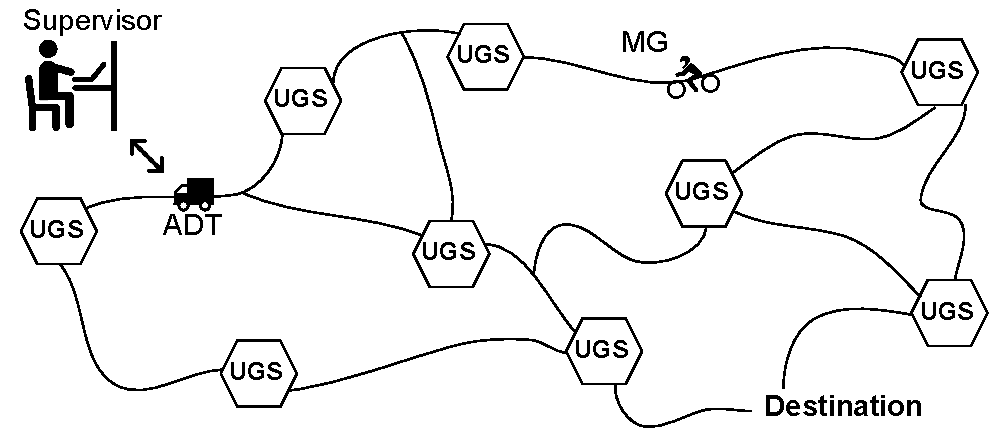
\includegraphics[width=0.5\textwidth]{Figures/RoadNet}
    	\caption{ADT in road network evading MG with information from noisy UGS.} 
        \label{fig:RoadNet}
        \vspace{-0.2cm}
    \end{figure}    
    
\subsubsection{Donut Delivery Application} \label{sec:donut_delivery}
Consider a concrete grounding example called the `Donut Delivery' problem (based on a `VIP escort' scenario~\cite{Humphrey2012-lr}). As shown in Fig. \label{fig:RoadNet} , an autonomous donut delivery truck (ADT) navigates a road network in order to reach a delivery destination while avoiding a motorcycle gang (MG) that will steal the donuts if they cross paths with the delivery truck. The motorcycle gang's location is unknown but can be estimated using intermittent updates from unmanned ground sensors (UGS). The delivery truck's decision space involves selecting a sequence of discrete actions (i.e. go straight, turn left, turn right, go back, stay in place). The ADT motion, UGS readings, and MG behavior are stochastic, and the problems of decision making and sensing are strongly coupled: some trajectories through the network might allow the ADT to localize the MG before heading to the delivery destination but incur a high time penalty); other trajectories may afford rapid delivery with high MG location uncertainty but increase the risk of getting caught by the MG, which can take multiple paths. A human supervisor monitors the ADT during operation. The supervisor does not have detailed knowledge or control of the ADT -- but can interrogate its actions, and (based on whatever limited amount of information is provided to the supervisor) can provide `go' or `no go' commands to proceed with or abort the delivery operation before it commences. 
%, as well as potentially modify its decision making stance (`aggressively pursue exit' vs. `be very conservative and cautious') in order to better cope with the MG (which is sporadically observed and follows an unknown course). \nisar{modify last sentence -- just state go/no go?}

The physical states describing the combined motion of the ADT (whose states are always perfectly observable) and MG can be discretized in time and space to produce a Markov process model defined by some initial joint state probability distribution and joint state transition matrix, which depends on the steering actions taken by the ADT. The probability of obtaining `detection' and `no detection' data from each UGS given the true state of the MG can be modeled and used to update probabilistic beliefs about the state of the chaser. Finally, a reward function $R(x_k,u_k) = R_k$ can be specified for each time step $k$ to encode user preferences over the combined state of the ADT and MG, e.g. $R_k = -200$ for each time step the ADT is not co-located with the MG but not yet at the exit, $R_k= -2000$ if the ADT and MG are co-located, and $R_k=+2000$ if the ADT reaches the exit without getting caught. Given these elements, the ADT's navigational planning and decision-making problem may be generally formulated as a POMDP. If the MG's state is fully observable at each step $k$ (e.g. due to very reliable and accurate UGS that cover all areas of the road network), the problem reduces to an MDP. 

%
%
%
%%
%
%
% %%%----old top part of background/related work (moved to intro)-------%%
% %%This section reviews several key concepts and related works which set the stage for our proposed computational machine self-confidence framework. To make the concepts discussed throughout the paper concrete and provide an accessible proof-of-concept testbed in later sections, we also describe a motivating APS application example inspired by ongoing research in unmanned robotic systems.  

% %%\subsection{Autonomous Systems and User Trust}
% %\nisar{for me todo: trim down and merge this section quite a bit -- may not really need all these subsections...can also probably significantly reduce/remove 2.1 stuff on trust [consider keeping/revising for RSS], just need to mention assurances and general idea of s/c very briefly before reviewing Famsec briefly, then move onto factors, examples, expts, results...}
% %An APS is generally any physical agent comprised of a machine controlled by some form of software-based autonomy. 
% Autonomy defines the ability of a physical system to perform a complex set of tasks with little/no human supervisory intervention for extended periods of time. This requires least one or more of the capabilities of an artificially intelligent physical agent, i.e. reasoning, knowledge representation, planning, learning, perception, motion/manipulation, and communication \cite{Israelsen2017-ym}. 
% %Despite many popular myths and misconceptions, 
% Yet, an autonomous physical system (APS) always interacts with a human user in some way \cite{Bradshaw2013-ck}.  That is, the aforementioned capabilities are only the means by which an APS achieves some \emph{intended} degree of self-sufficiency and self-directedness for tasks \emph{delegated} by a user to meet an `intent frame' (desired set of goals, plans, constraints, stipulations, and/or value statements) \cite{Miller2014-av}. 
% But as these capabilities have continued to improve and find new applications in recent years, the resulting APS are also becoming more complex, opaque and difficult for users (as well as designers,  certifying authorities, and other stakeholders) to fully comprehend. In particular, for APS characterized by state of the art uncertainty-based AI and data-driven machine learning, it can become extremely difficult to make precise predictions about behavior and performance limits with respect to desired intent frames in noisy, untested, and `out of scope' task conditions. 

% %Formal verification and validation tools could be used to tackle these issues at design time, but do not provide assurances that can be readily conveyed to or understood by (non-expert) users at run-time. 
% %%One may even argue that the task of assessing APS competency at run-time is a task so complex and burdensome in and of itself that it should also be delegated to the APS. 
% This ushers in questions related to user trust in autonomous systems, i.e. a user's willingness and security in depending on an APS to carry out a delegated set of tasks, having taken into consideration its characteristics and capabilities. 
% We focus here on the problem of how an APS can be designed to actively assist users in appropriately calibrating their trust in the APS. As surveyed in \cite{Israelsen2017-ym}, several broad classes of \emph{algorithmic assurances} for APS have been developed, where an assurance is defined as any property or behavior that can serve to increase or decrease a user's trust. 
% Good assurances are challenging to develop because they must allow users to gain better insight and understanding of APS behaviors for effectively managing operations, without undermining autonomous operations or burdening users in the process. 

% %%Taking out parags below, since these were aimed at FAT* folks...consider keeping/modifying for RSS? Need to include other more robotics-oriented works though, e.g. Srinivasa's Trust-POMDPs(eye roll...) ...
% %Many assurance strategies, such as value alignment \cite{Dragan2014-gu} (where an APS adapts its behavioral objectives with a user's intent frame via interactive learning) and interpretable reasoning \cite{Ruping2006-xj} (where algorithmic capabilities for planning, learning, reasoning, etc. are made accessible and easy to understand for non-expert users) put the onus on the APS (and designers) to integrate naturally transparent trust-calibrating behaviors into core system functionality. 
% %Other strategies, such as those based on post hoc explanation for learning and reasoning systems \cite{Lacave2004-gq,Ribeiro2016-uc} and data visualization \cite{Sacha2017-hf}, require users to render their own judgments via processing of information provided by the APS (possibly in response to specific user queries). 
% %Indeed, while the full range of assurance design strategies for APS have much in common with techniques for ensuring transparency and accountability for more general AI and learning systems, assurances based on self-monitoring offer an especially promising path for APS competency assessment. 

% %%\subsection{Self-Monitoring and Self-Confidence}
% % State of the art statistical machine learning and AI methods have ushered in major improvements to APS capabilities in recent years. 
% % Yet, as these methods and capabilities continue to improve and find new high-consequence applications, resulting APS implementations are also becoming more complex, opaque and difficult for users (as well as designers and certifying authorities) to fully comprehend. 
% % In particular, for sophisticated APS characterized by uncertainty-based reasoning and data-driven learning, it can become extremely difficult to make precise predictions about APS behavior and performance limits in noisy, untested, and `out of scope' task conditions with any degree of certainty. Formal verification and validation tools could be used to tackle these issues at design time, but do not provide assurances that can be readily conveyed to or understood by (non-expert) users at run-time. 
% % It can thus be argued that the task of assessing APS competency at run-time is in general so complex and burdensome that it should also be delegated to the APS itself. 

% %This leads to consideration of algorithmic self-monitoring methods, e.g. for introspective reasoning and learning \cite{Huang2017-lk}, and for fault diagnosis and computational meta-reasoning and meta-learning \cite{grant2018recasting} \nisar{fix broken ref?}. While promising for a variety of applications, these methods depend heavily on task outcome and performance assessments, and require data intensive evaluations. As such, they are best-suited to APS with narrow, well-defined capabilities and few computational resource constraints. However, many current and future APS must operate in open-ended task settings in physical environments with significant computational limitations, e.g. due to constrained platform size, weight, power, etc. or limited test and evaluation opportunities. 
% %The interpretation of `favorable vs. unfavorable' task outcomes can also shift in subtle yet significant ways that may not be obvious to non-expert users, depending on the interactions of designed APS capabilities and task context (all of which may also change drastically over the course of a given operational instance). 

% These limitations motivate \emph{process-based assessment} techniques that allow APS to more generally self-qualify their capabilities and competency boundaries by evaluating and reporting their associated degree of `self-trust' or \emph{self-confidence} for a particular task. 
% This resonates with the concepts put forth by \cite{Hutchins2015-if}, which proposed using human expert evaluations of specific APS capabilities to manually encode where and when these may break down in particular tasking situations. However, to be useful in real applications, APS must be able to form these evaluations on their own. 
% %As evidenced by recent work in neurocomputational modeling of decision-making for visual-motor tasks, self-confidence reporting in humans generally requires second-order reasoning about uncertainties associated with particular task outcomes, i.e. assessments of `uncertainties in uncertainty' as well as of one's own reasoning processes \cite{Adler2016-oi}. 
% To this end, several formal definitions and algorithmic techniques for allowing APS to automatically compute their own machine self-confidence scores in the context of different tasks and uncertainty-based capability assessments have been proposed recently \cite{Sweet2016-tz, Israelsen2017-ym}. 
% %For instance, Kuter and Miller \cite{Kuter2015-qh} proposed to evaluate \emph{plan stability} for systems that rely on hierarchical task planning algorithms, using formal counter-planning and plan-repair methods to mitigate threatening contingencies for a given plan. 
% %This relies heavily on fixed knowledge bases and ontologies, and so only supports assessments for well-understood environments, tasks, systems, and contexts. 
% %These and other approaches are reviewed in \cite{Sweet2016-tz}, as well as in \cite{Israelsen2017-ym} in the context of algorithmic interactions for human-autonomous system trust relationships. 
% For the sake of brevity, we restrict attention to the definition of self-confidence used in this work: \textbf{An agent's perceived ability to achieve assigned goals (within a defined region of autonomous behavior) after accounting for (1) uncertainties in its knowledge of the world, (2) uncertainties of its own state, and (3) uncertainties about its reasoning process and execution abilities.} However, even with this definition, a framework for computing and communicating self-confidence for general decision-making autonomy architectures has not yet been established, and studies have not yet been conducted to investigate whether machine self-confidence reporting promotes appropriate usage and user trust of APS. This work provides results aimed at addressing both these gaps. 
